\documentclass[journal]{IEEEtran}
\usepackage[a5paper, margin=10mm, onecolumn]{geometry}
\usepackage{tfrupee} % Include tfrupee package

\setlength{\headheight}{1cm} % Set the height of the header box
\setlength{\headsep}{0mm}     % Set the distance between the header box and the top of the text

\usepackage{gvv-book}
\usepackage{gvv}
\usepackage{cite}
\usepackage{amsmath,amssymb,amsfonts,amsthm}
\usepackage{algorithmic}
\usepackage{graphicx}
\usepackage{textcomp}
\usepackage{xcolor}
\usepackage{txfonts}
\usepackage{listings}
\usepackage{enumitem}
\usepackage{mathtools}
\usepackage{gensymb}
\usepackage{comment}
\usepackage[breaklinks=true]{hyperref}
\usepackage{tikz}
\usepackage{tkz-euclide} 
\usepackage{pgfplots}
\usepackage[latin1]{inputenc}                                
\usepackage{color}                                            
\usepackage{array}                                            
\usepackage{longtable}                                       
\usepackage{calc}                                             
\usepackage{multirow}                                         
\usepackage{hhline}                                           
\usepackage{ifthen}                                           
\usepackage{lscape}

\begin{document}

\bibliographystyle{IEEEtran}
\vspace{3cm}

\title{9.3.12.A}
\author{EE24BTECH11026 - G.Srihaas}
{\let\newpage\relax\maketitle}

\renewcommand{\thefigure}{\theenumi}
\renewcommand{\thetable}{\theenumi}
\setlength{\intextsep}{10pt} % Space between text and floats

\numberwithin{equation}{enumi}
\numberwithin{figure}{enumi}
\renewcommand{\thetable}{\theenumi}

\textbf{QUESTION} \\
Find all points of local maxima and local minima of the function $f$ given by
\begin{align}
f(x) &= x^3 - 3x + 3.
\end{align}

\solution
\textbf{THEORETICAL METHOD} \\
We can find the local maximum and minimum of the polynomial function $f(x)$ using the first and second derivatives. \\
The first derivative helps to identify the stationary points, i.e., the points where the function is maximum or minimum. \\
The second derivative helps to identify if we get a maximum or minimum at the said stationary points. \\

\begin{align}
f(x) &= x^3 - 3x + 3, \\
f^{\prime}(x) &= 3x^2 - 3 = 3(x - 1)(x + 1), \\
f^{\prime}(x) &= 0, \\
x &= 1, \\
x &= -1.
\end{align}

Hence, the stationary points are $-1$ and $1$. Now finding the second derivative: \\
\begin{align}
f^{\prime\prime}(x) &= 6x, \\
f^{\prime\prime}(-1) &= 6(-1) = -6 < 0, \\
f^{\prime\prime}(1) &= 6(1) = 6 > 0.
\end{align}

Thus:
\begin{itemize}
    \item At $x = -1$, $f^{\prime\prime}(-1) < 0$, so there is a local maximum.
    \item At $x = 1$, $f^{\prime\prime}(1) > 0$, so there is a local minimum.
\end{itemize}

$\therefore$ The point of local maximum is $x = -1$, and the point of local minimum is $x = 1$.\\

\textbf{COMPUTATIONAL LOGIC}:Gradient descent method\\

Gradient descent is an iterative optimization algorithm used to find the minimum or maximum of a function by iteratively adjusting the input value in the direction of the steepest descent (for minimum) or ascent (for maximum). It is widely used in machine learning and optimization problems, particularly when dealing with differentiable functions.

Here we will apply the gradient descent method to find the local minima and maxima of the cubic function:
\begin{align}
f(x) &= x^3 - 3x + 3
\end{align}

Gradient Descent Method:\\

The update rule for gradient descent is given by the difference equation:
\begin{align}
x_{n+1} &= x_n - \eta.f^{\prime}(x_n)
\end{align}
where:
\begin{itemize}
    \item $ x_n $ is the current value of $ x $,
    \item $ x_{n+1} $ is the updated value of $ x $,
    \item $ \eta $ is the learning rate (a small positive constant),
    \item $ f^{\prime}(x_n) $ is the derivative of the function $ f(x) $ evaluated at $ x_n $, also called the gradient.
\end{itemize}

e initialize the algorithm with starting points near these values and observe convergence to the critical points.

\textbf{Gradient Descent Algorithm:}
\begin{itemize}
    \item Initialize \( x_0 \) 
    \item Update \( x \) iteratively using the formula:
    \begin{align}
    x_{n+1} &= x_n - \eta.(3x_n^2 - 3)\\
    x_{n+1} &=(-3\eta)x_n^2 + x_n + 3\eta
    \end{align}
    until the change in \( x \) is smaller than a chosen threshold.
    \item The algorithm stops when \( |x_{n+1} - x_n| \) is sufficiently small.
\end{itemize}

\textbf{Critical Points Obtained:}
\begin{itemize}
    \item The local minimum occurs at \( x = 1 \).
    \item The local maximum occurs at \( x = -1 \).
\end{itemize}

\begin{figure}[ht]
	\centering
	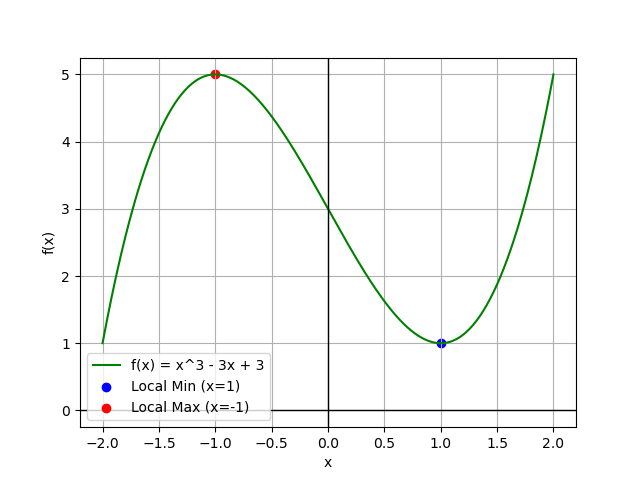
\includegraphics[width=1\textwidth]{figs/fig.png}
	\label{fig:Plot1}
\end{figure}

\end{document}

